\documentclass[12pt,]{article}
\usepackage{lmodern}
\usepackage{amssymb,amsmath,stmaryrd}
\usepackage{ifxetex,ifluatex}
\usepackage{fixltx2e} % provides \textsubscript
\ifnum 0\ifxetex 1\fi\ifluatex 1\fi=0 % if pdftex
  \usepackage[T1]{fontenc}
  \usepackage[utf8]{inputenc}
\else % if luatex or xelatex
  \ifxetex
    \usepackage{mathspec}
  \else
    \usepackage{fontspec}
  \fi
  \defaultfontfeatures{Ligatures=TeX,Scale=MatchLowercase}
\fi
% use upquote if available, for straight quotes in verbatim environments
\IfFileExists{upquote.sty}{\usepackage{upquote}}{}
% use microtype if available
\IfFileExists{microtype.sty}{%
\usepackage{microtype}
\UseMicrotypeSet[protrusion]{basicmath} % disable protrusion for tt fonts
}{}
\usepackage[margin=1in]{geometry}
\usepackage{hyperref}
\PassOptionsToPackage{usenames,dvipsnames}{color} % color is loaded by hyperref
\hypersetup{unicode=true,
            pdftitle={Extending ggplot2 for linked and animated web graphics},
            pdfkeywords={Animation, Multiple linked views, Statistical graphics, Exploratory data
analysis, Web technologies, Grammar of graphics},
            colorlinks=true,
            linkcolor=cyan,
            citecolor=black,
            urlcolor=Blue,
            breaklinks=true}
\urlstyle{same}  % don't use monospace font for urls
\usepackage{color}
\usepackage{fancyvrb}
\newcommand{\VerbBar}{|}
\newcommand{\VERB}{\Verb[commandchars=\\\{\}]}
\DefineVerbatimEnvironment{Highlighting}{Verbatim}{commandchars=\\\{\}}
% Add ',fontsize=\small' for more characters per line
\usepackage{framed}
\definecolor{shadecolor}{RGB}{248,248,248}
\newenvironment{Shaded}{\begin{snugshade}}{\end{snugshade}}
\newcommand{\AlertTok}[1]{\textcolor[rgb]{0.94,0.16,0.16}{#1}}
\newcommand{\AnnotationTok}[1]{\textcolor[rgb]{0.56,0.35,0.01}{\textbf{\textit{#1}}}}
\newcommand{\AttributeTok}[1]{\textcolor[rgb]{0.77,0.63,0.00}{#1}}
\newcommand{\BaseNTok}[1]{\textcolor[rgb]{0.00,0.00,0.81}{#1}}
\newcommand{\BuiltInTok}[1]{#1}
\newcommand{\CharTok}[1]{\textcolor[rgb]{0.31,0.60,0.02}{#1}}
\newcommand{\CommentTok}[1]{\textcolor[rgb]{0.56,0.35,0.01}{\textit{#1}}}
\newcommand{\CommentVarTok}[1]{\textcolor[rgb]{0.56,0.35,0.01}{\textbf{\textit{#1}}}}
\newcommand{\ConstantTok}[1]{\textcolor[rgb]{0.00,0.00,0.00}{#1}}
\newcommand{\ControlFlowTok}[1]{\textcolor[rgb]{0.13,0.29,0.53}{\textbf{#1}}}
\newcommand{\DataTypeTok}[1]{\textcolor[rgb]{0.13,0.29,0.53}{#1}}
\newcommand{\DecValTok}[1]{\textcolor[rgb]{0.00,0.00,0.81}{#1}}
\newcommand{\DocumentationTok}[1]{\textcolor[rgb]{0.56,0.35,0.01}{\textbf{\textit{#1}}}}
\newcommand{\ErrorTok}[1]{\textcolor[rgb]{0.64,0.00,0.00}{\textbf{#1}}}
\newcommand{\ExtensionTok}[1]{#1}
\newcommand{\FloatTok}[1]{\textcolor[rgb]{0.00,0.00,0.81}{#1}}
\newcommand{\FunctionTok}[1]{\textcolor[rgb]{0.00,0.00,0.00}{#1}}
\newcommand{\ImportTok}[1]{#1}
\newcommand{\InformationTok}[1]{\textcolor[rgb]{0.56,0.35,0.01}{\textbf{\textit{#1}}}}
\newcommand{\KeywordTok}[1]{\textcolor[rgb]{0.13,0.29,0.53}{\textbf{#1}}}
\newcommand{\NormalTok}[1]{#1}
\newcommand{\OperatorTok}[1]{\textcolor[rgb]{0.81,0.36,0.00}{\textbf{#1}}}
\newcommand{\OtherTok}[1]{\textcolor[rgb]{0.56,0.35,0.01}{#1}}
\newcommand{\PreprocessorTok}[1]{\textcolor[rgb]{0.56,0.35,0.01}{\textit{#1}}}
\newcommand{\RegionMarkerTok}[1]{#1}
\newcommand{\SpecialCharTok}[1]{\textcolor[rgb]{0.00,0.00,0.00}{#1}}
\newcommand{\SpecialStringTok}[1]{\textcolor[rgb]{0.31,0.60,0.02}{#1}}
\newcommand{\StringTok}[1]{\textcolor[rgb]{0.31,0.60,0.02}{#1}}
\newcommand{\VariableTok}[1]{\textcolor[rgb]{0.00,0.00,0.00}{#1}}
\newcommand{\VerbatimStringTok}[1]{\textcolor[rgb]{0.31,0.60,0.02}{#1}}
\newcommand{\WarningTok}[1]{\textcolor[rgb]{0.56,0.35,0.01}{\textbf{\textit{#1}}}}
\usepackage{longtable,booktabs}
\usepackage{graphicx,grffile}
\makeatletter
\def\maxwidth{\ifdim\Gin@nat@width>\linewidth\linewidth\else\Gin@nat@width\fi}
\def\maxheight{\ifdim\Gin@nat@height>\textheight\textheight\else\Gin@nat@height\fi}
\makeatother
% Scale images if necessary, so that they will not overflow the page
% margins by default, and it is still possible to overwrite the defaults
% using explicit options in \includegraphics[width, height, ...]{}
\setkeys{Gin}{width=\maxwidth,height=\maxheight,keepaspectratio}
\IfFileExists{parskip.sty}{%
\usepackage{parskip}
}{% else
\setlength{\parindent}{0pt}
\setlength{\parskip}{6pt plus 2pt minus 1pt}
}
\setlength{\emergencystretch}{3em}  % prevent overfull lines
\providecommand{\tightlist}{%
  \setlength{\itemsep}{0pt}\setlength{\parskip}{0pt}}
\setcounter{secnumdepth}{5}
% Redefines (sub)paragraphs to behave more like sections
\ifx\paragraph\undefined\else
\let\oldparagraph\paragraph
\renewcommand{\paragraph}[1]{\oldparagraph{#1}\mbox{}}
\fi
\ifx\subparagraph\undefined\else
\let\oldsubparagraph\subparagraph
\renewcommand{\subparagraph}[1]{\oldsubparagraph{#1}\mbox{}}
\fi

%%% Use protect on footnotes to avoid problems with footnotes in titles
\let\rmarkdownfootnote\footnote%
\def\footnote{\protect\rmarkdownfootnote}

% ------------------------------------------------------------------------------
% Start of JCGS specific titlepage
% ------------------------------------------------------------------------------

\usepackage{tabularx}

\usepackage{amsthm}
\newtheorem{theorem}{Theorem}[section]
\newtheorem{lemma}{Lemma}[section]
\theoremstyle{definition}
\newtheorem{definition}{Definition}[section]
\newtheorem{corollary}{Corollary}[section]
\newtheorem{proposition}{Proposition}[section]
\theoremstyle{definition}
\newtheorem{example}{Example}[section]
\theoremstyle{definition}
\newtheorem{exercise}{Exercise}[section]
\theoremstyle{remark}
\newtheorem*{remark}{Remark}
\newtheorem*{solution}{Solution}
\begin{document}

\def\spacingset#1{\renewcommand{\baselinestretch}%
{#1}\small\normalsize} \spacingset{1}

\title{\bf Extending ggplot2 for linked and animated web graphics}
\author{
  Carson Sievert \\ 
  Department of Statistics, Iowa State University \\
  Susan VanderPlas \\
  Department of Statistics, Iowa State University \\
  Jun Cai \\
  Department of Earth System Science, Tsinghua University\\
  Kevin Ferris \\
  Baseball Operations Department, Tampa Bay Rays \\
  Faizan Uddin Fahad Khan \\
  Department of Computer Science \& Engineering, IIT BHU \\
  Toby Dylan Hocking \\ 
  Department of Human Genetics, McGill University \\
}
\maketitle

\bigskip
\begin{abstract}
% 200 or fewer words
Interactive web graphics are great for communication and knowledge
sharing, but are difficult to leverage during the exploratory phase of a
data science workflow. Even before the web, interactive graphics helped
data analysts quickly gather insight from data, discover the unexpected,
and develop better model diagnostics. Web technologies, however, are not
designed to fit inside an exploratory data analysis (EDA) workflow where
rapid iteration between data manipulation, modeling, and visualization
must occur. We propose the R package \textbf{animint} for rapid creation
of linked and animated web graphics through a simple extension of
\textbf{ggplot2}'s implementation of the Grammar of Graphics. The
extension uses the existing \textbf{ggplot2} code, and leverages a
simple API for describing animations and graphical queries between
multiple linked views in a standalone web page.
\end{abstract}

\noindent
{\it Keywords:}  Animation, Multiple linked views, Statistical graphics, Exploratory data
analysis, Web technologies, Grammar of graphics
\vfill

\newpage
\spacingset{1.45} % DON'T change the spacing!

% ------------------------------------------------------------------------------
% End of JCGS specific titlepage
% ------------------------------------------------------------------------------

\hypertarget{intro}{%
\section{Introduction}\label{intro}}

For more than a half century now, statisticians have designed, built,
and used interactive graphics for exploring high-dimensional data and
better informing their modeling process. In fact, the ASA maintains a
video library (\url{http://stat-graphics.org/movies/}) to document and
demonstrate applications of instrumental interactive statistical
graphics systems such as \texttt{PRIM-9} (Fisherkeller and Tukey 1988),
\texttt{Data\ Viewer} (Andreas Buja and McDonald 1988), \texttt{XGobi}
(Swayne, Cook, and Buja 1998), \texttt{GGobi} (D. Cook and Swayne 2007),
and \texttt{Mondrian} (Theus 2002). These, as well as other influential
systems, such as \texttt{LISP-STAT} (Tierney 1990) and \texttt{MANET}
(Unwin A. 1996), all have a rich support for accomplishing a wide
variety of statistical analysis tasks, and most were developed before
the web browser had rich graphics support.

All of these systems, as well as some more modern systems, such as
\textbf{rggobi} (Duncan Temple Lang 2016), \textbf{iplots} (Urbanek
2011), \textbf{loon} (Waddell and Oldford 2018), etc, require a heavy
set of computational dependencies in order to view or interact with
graphics. These requirements grant the freedom to leverage libraries
with sophisticated statistical functionality on-demand, but it limits
the ability to share or embed such graphics in a larger document. Some
of these systems allow users to create the graphics from the
command-line, which as Unwin and Hofmann (2009) points out, allows power
users to combine the strengths of a programming interface (e.g.,
precise, repeatable, fast, and extensible) with the strengths of a
graphical interface (e.g., intuitive, forgiving, and easy-to-use). Web
technologies can certainly be used to build a similar class of system,
but in order to capitalize on the key strength of web technologies
(e.g., accessible, portable, and composable), we must be mindful if
which technologies we're requiring in such a system, and minimize those
requirements whenever possible.

Generally speaking, web graphics that use purely client-side
technologies (i.e., \texttt{HTML}, \texttt{SVG}, \texttt{CSS}, and
\texttt{JavaScript}) are desired over client-server web applications
because of their relative ease of distribution and maintenance. This is
why many web-based graphing libraries work entirely with client-side
technologies, like Vega (Trifacta 2014) and plotly.js (Plotly 2015).\\
Unfortunately, client-side technologies are not particularly well-suited
for statistical computation, which we often want to leverage via dynamic
controls in an interactive statistical graphics system. In this
scenario, it often makes sense to introduce a client-server
infrastructure to leverage functionality that is not natively supported
by web browsers (e.g., R, python, etc).

Focusing just on the R language, there are now numerous ways to develop
web applications, including the R package \textbf{shiny} (RStudio 2013),
which makes it easy for R users to take their existing scripting
workflow and wrap a web interface around it. \textbf{Shiny} is great for
quickly prototyping interactive webpages that re-execute R code
on-demand, but that flexibility comes at the cost of requiring a complex
web server framework, which can be hard to scale, maintain, and secure
sensitive information. Unfortunately, all too often, a web application
framework is used to implement linked and animated graphics that could
more easily be described with an idiomatic R interface which produces a
purely client-side result.

There are now a large number of R packages that interface with purely
client-side graphing libraries and give users the option of embedding
these graphics in a larger web application. In fact, this is a large
enough use case that the R package \textbf{htmlwidgets} (Vaidyanathan et
al. 2018) was created to make it easier to get these interfaces to work
seamlessly in any context (e.g., \textbf{shiny}, \textbf{rmarkdown},
RStudio, R prompt, Jupyter notebook, etc). In our experience, these R
packages rarely provide a way to describe linked views in R and produce
a purely client-side result, which we view as a powerful workflow for
exploratory web graphics.

We propose an extension of \textbf{ggplot2}'s layered Grammar of
Graphics API to create interactive web graphics that don't require
server-side technologies. The core idea lies in attaching metadata to
graphical marks that can be used to hide/show subsets of data. The
resulting framework is quite similar to what D. Cook, Buja, and Swayne
(2007) describe as brushing in multiple linked views as a database
query. The assignment of data to graphical marks is done through
\emph{aesthetic mappings}, which is a term the Grammar of Graphics uses
for mapping data to visual attributes (e.g., color, shape, x, y, etc).
Typically aesthetic mappings are visual, meaning they can be easily seen
in a static graphic, but our proposed variable mappings are more
conceptual, meaning that they can't easily be seen, but can be used to
control certain interactive properties. To give a small example, Figure
\ref{fig:tips} depicts a graphical query made by assigning sensible
metadata to graphical marks via the \texttt{clickSelects} and
\texttt{showSelected} aesthetics.

In addition to graphical queries, our extension supports a number of
other interactive features, including animation, tooltips, and
hyperlinks. A summary of these extensions and relevant additional
options are provided in Table \ref{tab:overview}. There are a number of
other options specific to our implementation in the R package
\textbf{animint} which are described in the supplemental materials.

\begin{table}

\caption{
New features that animint adds to the grammar of graphics.
}\label{tab:overview}
\small
\begin{tabularx}{\textwidth}{|l|l|l|}
\hline
Feature & Type & Description \\
\hline
\texttt{clickSelects} & aesthetic & value(s) to select on click \\
\texttt{showSelected} & aesthetic & value(s) attached to mark(s) that determine when they are shown  \\
\texttt{key} & aesthetic & value(s) attached to mark(s) for smooth transitions. \\
\texttt{tooltip} & aesthetic & information to display on hover \\
\texttt{href} & aesthetic & URL link to open on click \\
\texttt{first} & option & what value(s) should be selected by default?  \\
\texttt{time} & option & delay between animation frames.  \\
\texttt{duration} & option & to specify smooth transitions.  \\
\texttt{selector.types} & option & should selections accumulate?  \\
\texttt{selectize} & option & include a dropdown widget to set selection value(s) indirectly? \\
\hline
\end{tabularx}

\end{table}

\hypertarget{related-work}{%
\section{Related work}\label{related-work}}

It is important to acknowledge that \textbf{ggplot2} is built on top of
the R package \textbf{grid}, a low-level graphics system, which is now
bundled with R itself (R Core Team 2017). Neither \textbf{grid}, nor
\textbf{base} R graphics, have strong support for handling user
interaction, which creates a need for add-on packages. There are a
number of approaches these packages take to rendering, each with their
own benefits and drawbacks. Traditionally, they build on low-level R
interfaces to graphical systems such as GTK+ (Lawrence and Temple Lang
2010), Qt (Lawrence and Sarkar 2016), or Java GUI frameworks (Urbanek
2016). In general, the resulting system can be very fast and flexible,
but sharing and reproducing output is usually a problem due to the heavy
software requirements. Although there may be sacrifices in performance,
using the modern web browser as a canvas is more portable, accessible,
and composable (graphics can be embedded within larger
frameworks/documents).

Base R does provide a Scalable Vector Graphics (SVG) device,
\texttt{svg()}, via the Cairo graphics API (Cairo 2016). The R package
\textbf{SVGAnnotation} provides functionality to post-process
\texttt{svg()} output in order to add interactive and dynamic features
(Nolan and Lang 2012). This is a powerful approach, since in theory it
can work with any R graphic, but the package is self-described as a
proof-of-concept which reverse-engineers poorly-structured
\texttt{svg()} output. As a result, it is not straightforward to extend
this system for linked data visualizations with advanced functionality
(multiple layers, multiple plots, multiple selection variables).

The lack of well-structured SVG for R graphics motivated the
\textbf{gridSVG} package which provides sensible structuring of SVG
output for grid graphics (Murrell and Potter 2015). This package also
provides some low-level tools for animating or adding interactive
features, where grid objects must be referenced by name. As a result,
use of this interface to add interactivity to a \textbf{ggplot2} plot
requires understanding of the grid naming scheme \textbf{ggplot2} uses
internally. An interface where interactivity can be expressed by
referencing the data to be visualized, rather than the building blocks
of the graphics system, would be preferable since the former interface
is decoupled from the implementation and does not require knowledge of
grid.

In terms of the animation API, the R package \textbf{gganimate} is very
similar to our system (Robinson 2016). It directly extends
\textbf{ggplot2} by adding a new aesthetic, named \texttt{frame}, which
splits the data into subsets (one for each unique value of the frame
variable), produces a static plot for each subset, and uses the
\textbf{animation} package to combine the images into a key frame
animation (Xie 2013). This is quite similar but not as flexible as our
system's support for animation, which we fully describe in Section
\ref{animation}. Either system has the ability to control the amount of
time that a given frame is displayed, but our system can also animate
the transition between frames via the \texttt{d3.transition()} API
(Bostock, Oglevetsky, and Heer 2011). Smooth transitions help the
animation viewer track positions between frames, which is useful in many
scenarios, such as the touring example discussed in Section \ref{tour}.
The \textbf{tweenr} package provides similar smooth transitions, by
computing data values in R that interpolate between animation frames (in
\textbf{animint}, these calculations are performed in the web browser).

The \textbf{ggvis} package is similar to our system in that is also
inspired by the Grammar of Graphics (Chang and Wickham 2015). It does
not directly extend \textbf{ggplot2}, but instead provides a brand new
purely functional interface which is designed with interactive graphics
in mind. It currently relies on Vega to render the SVG graphics from
JSON (Trifacta 2014), and the R package \textbf{shiny} to enable many of
its interactive capabilities (RStudio 2013). The interface gives
tremendous power to R users, as it allows one to write R functions to
handle user events. This power does come with a cost, though, as sharing
and hosting \textbf{ggvis} graphics typically require special web server
softwares, even when the interaction logic could be handled entirely
client-side.

The tour is a useful visualization technique for exploring
high-dimensional data which requires interactive and dynamic graphics.
The open-source software ggobi is currently the most fully-featured
toolkit for touring data and has support for interactive techniques such
as linking, zooming, panning, and identifying (D. Cook and Swayne 2007).
The R package \textbf{rggobi} (Duncan Temple Lang 2016) provides an R
interface to ggobi's graphical interface, but it unfortunately has many
software requirements. Furthermore, sharing the interactive versions of
these graphics are not possible. The R package \textbf{cranvas} aims to
be the successor to ggobi, with support for similar interactive
techniques, but with a more flexible interface for describing plots
inspired by the Grammar of Graphics (Xie et al. 2013). \textbf{Cranvas}
also has many software requirements which limits its portability and
accessibility.

Another R package for interactive graphics is \textbf{iplots} (Urbanek
2011), which has several important differences compared to
\textbf{animint}. Brushing/highlighting of linked iplots is supported
for single-layer plots such as scatterplots or barplots, but it is not
easy to define new multi-layer interactive plots. Furthermore since
iplots does not use the Grammar of Graphics, it is difficult to create
legends and multi-panel plots. Finally since iplots requires compiled
C++ code for rendering on the local machine, its graphics are not as
easy to share as \textbf{animint} graphics which can be viewed in a web
browser.

\hypertarget{extending-the-layered-grammar-of-graphics}{%
\section{Extending the layered grammar of
graphics}\label{extending-the-layered-grammar-of-graphics}}

In this section, we describe in detail our extension of
\textbf{ggplot2}'s layered grammar of graphics implementation (Wickham
2010). In \textbf{ggplot2}, there are five essential components that
define a layer of graphical makings: data, mappings (i.e., aesthetics),
geometry, statistic, and position. These simple components are easy to
understand in isolation and can be combined in many ways to express a
wide array of graphics. For a simple example, here is one way to create
a scatterplot in \textbf{ggplot2} of variables named
\texttt{\textless{}X\textgreater{}} and
\texttt{\textless{}Y\textgreater{}} in
\texttt{\textless{}DATA\textgreater{}}:

\begin{Shaded}
\begin{Highlighting}[]
\KeywordTok{ggplot}\NormalTok{() }\OperatorTok{+}\StringTok{ }\KeywordTok{layer}\NormalTok{(}
  \DataTypeTok{data =} \OperatorTok{<}\NormalTok{DATA}\OperatorTok{>}\NormalTok{, }
  \DataTypeTok{mapping =} \KeywordTok{aes}\NormalTok{(}\DataTypeTok{x =} \OperatorTok{<}\NormalTok{X}\OperatorTok{>}\NormalTok{, }\DataTypeTok{y =} \OperatorTok{<}\NormalTok{Y}\OperatorTok{>}\NormalTok{), }
  \DataTypeTok{geom =} \StringTok{"point"}\NormalTok{, }
  \DataTypeTok{stat =} \StringTok{"identity"}\NormalTok{,}
  \DataTypeTok{position =} \StringTok{"identity"}
\NormalTok{)}
\end{Highlighting}
\end{Shaded}

For every geometry, \textbf{ggplot2} provides a convenient wrapper
around \texttt{layer()} which provides sensible defaults for the
statistic and position (in this case, both are ``identity''):

\begin{Shaded}
\begin{Highlighting}[]
\KeywordTok{ggplot}\NormalTok{() }\OperatorTok{+}\StringTok{ }\KeywordTok{geom_point}\NormalTok{(}
  \DataTypeTok{data =} \OperatorTok{<}\NormalTok{DATA}\OperatorTok{>}\NormalTok{, }
  \KeywordTok{aes}\NormalTok{(}\DataTypeTok{x =} \OperatorTok{<}\NormalTok{X}\OperatorTok{>}\NormalTok{, }\DataTypeTok{y =} \OperatorTok{<}\NormalTok{Y}\OperatorTok{>}\NormalTok{)}
\NormalTok{)}
\end{Highlighting}
\end{Shaded}

A single \textbf{ggplot2} plot can be comprised of multiple layers, and
different layers can correspond to different data. Since each graphical
mark within a \textbf{ggplot2} layer corresponds to one (or more)
observations in \texttt{\textless{}DATA\textgreater{}}, aesthetic
mappings provide a mechanism for mapping graphical selections to the
original data (and vice-versa) which is essential to any interactive
graphics system (Wickham et al. 2010). Thus, given a way to combine
multiple \textbf{ggplot2} plots into a single view, this design can be
extended to support a notion of multiple linked views, as those
discussed by Ahlberg, Williamson, and Shneiderman (1991) and Buja et al.
(1991).

\hypertarget{extension}{%
\subsection{Linking views via aesthetic mappings}\label{extension}}

D. Cook and Swayne (2007) use \texttt{SQL} queries to formalize the
linked views infrastructure discussed in Ahlberg, Williamson, and
Shneiderman (1991) and Buja et al. (1991). We use a similar approach to
show how aesthetic mappings can be used to assign data values to
graphical marks via \textbf{ggplot2} to support similar graphical
queries. It's worth noting that, since these aesthetics effectively
define a set of database queries that are known at print time, these
queries can be made by direct manipulation of graphical marks and/or
indirect manipulation via a dropdown widget, as discussed in Section
\ref{direction}. It's also worth noting that these aesthetics could be
defined in such a way that they are not solely restricted to any
particular user event (e.g.~mouse click), but for sake of demonstration,
we restrict focus to our \textbf{animint} implementation, which has
\texttt{clickSelects} and \texttt{showSelected} aesthetics. Consider the
R code below which uses these aesthetics to describe the interactive
graphic shown in Figure \ref{fig:tips}\footnote{Interactive versions
of all of the figures mentioned in this paper can be found at
\url{http://members.cbio.mines-paristech.fr/~thocking/animint-paper-figures/}}.

\begin{Shaded}
\begin{Highlighting}[]
\KeywordTok{data}\NormalTok{(tips, }\DataTypeTok{package =} \StringTok{"reshape2"}\NormalTok{)}
\NormalTok{bar <-}\StringTok{ }\KeywordTok{ggplot}\NormalTok{(tips) }\OperatorTok{+}\StringTok{ }
\StringTok{  }\KeywordTok{geom_bar}\NormalTok{(}\KeywordTok{aes}\NormalTok{(}\DataTypeTok{x =}\NormalTok{ sex, }\DataTypeTok{clickSelects =}\NormalTok{ sex))}
\NormalTok{scatter <-}\StringTok{ }\KeywordTok{ggplot}\NormalTok{(tips) }\OperatorTok{+}
\StringTok{  }\KeywordTok{geom_point}\NormalTok{(}\KeywordTok{aes}\NormalTok{(}\DataTypeTok{x =}\NormalTok{ total_bill, }\DataTypeTok{y =}\NormalTok{ tip), }\DataTypeTok{alpha =} \FloatTok{0.3}\NormalTok{) }\OperatorTok{+}
\StringTok{  }\KeywordTok{geom_point}\NormalTok{(}\KeywordTok{aes}\NormalTok{(}\DataTypeTok{x =}\NormalTok{ total_bill, }\DataTypeTok{y =}\NormalTok{ tip, }\DataTypeTok{showSelected =}\NormalTok{ sex))}
\end{Highlighting}
\end{Shaded}

The \texttt{clickSelects} aesthetic is used to declare a geom which can
be clicked to set selection value(s). For the example in Figure
\ref{fig:tips}, we declare a bar with \texttt{clickSelects=sex} and
refer to the current set of selection value(s) as
\texttt{selected\_sex}. The value of \texttt{selected\_sex} can take on
any subset of the unique values of \texttt{sex}, and in this case, the
unique values are \texttt{Male} and \texttt{Female}. The selection set,
\texttt{selected\_sex}, is then used to select subsets of data for geoms
with the \texttt{showSelected=sex} aesthetic. In this case there is a
geom point with \texttt{showSelected=sex}, so clicking on a bar results
in an update to the displayed subset of points.

\begin{figure}
\centering
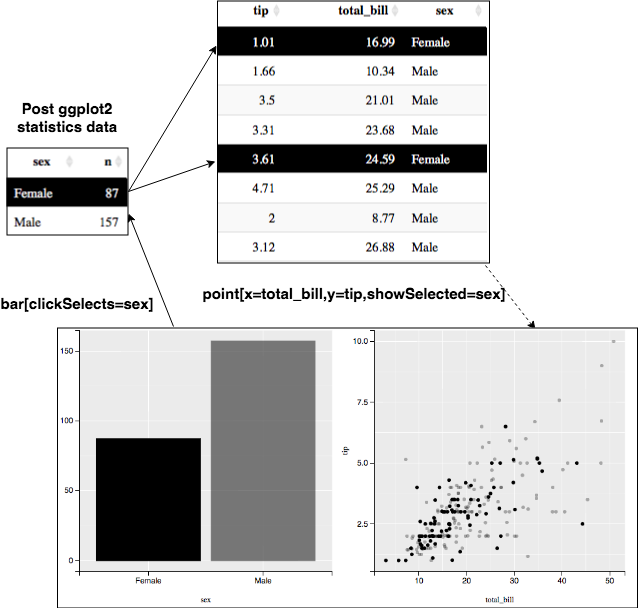
\includegraphics{images/tips}
\caption{\label{fig:tips}A graphical query of tips data set. Left: the
\texttt{clickSelects} aesthetic designates a clickable geom bar that can
change a selection variable. Right: the \texttt{showSelected} aesthetic
designates a geom point that responds by showing only the data which
corresponds to the current selection.}
\end{figure}

In the R code above, the \texttt{geom\_bar()} layer in the left-hand
plot is linked to the 2nd \texttt{geom\_point()} layer in the right-hand
plot since the \texttt{clickSelects} and \texttt{showSelected}
aesthetics are mapped to a common variable, \texttt{sex}. Note how the
first \texttt{geom\_point()} layer does not have a \texttt{showSelected}
mapping, but has a bit of alpha transparency, so all the data is shown
in light gray, and the current selection is portrayed in black. In other
words, when a bar is clicked, in order to update the second layer of
points, our system performs an SQL query of the form:

\begin{Shaded}
\begin{Highlighting}[]
\KeywordTok{SELECT}\NormalTok{ * }\KeywordTok{FROM}\NormalTok{ tips}
  \KeywordTok{WHERE}\NormalTok{ sex }\KeywordTok{IN}\NormalTok{ selected_sex}
\end{Highlighting}
\end{Shaded}

In this example, \texttt{selected\_sex} is either \texttt{Male} or
\texttt{Female} (a single selected value), but as we show in later
examples, a selection set can also be multiple values. Although the
\texttt{clickSelects} aesthetic is tied to a mouse click event, other
aesthetics could easily be created to support other selection events,
such as hover or click+drag. Statistically speaking, this type of
interaction is useful for navigating through joint distributions
conditional upon discrete values. In this sense, our extension is
closely related to trellis displays (Becker, Cleveland, and Shyu 2010)
and linked scatterplot brushing (Becker and Cleveland 1987). The major
differences are that our conditioning is layer-specific (not
plot-specific), is not tied to a particular geometry, and can be
controlled through direct manipulation or animation controls.

\hypertarget{worldbank}{%
\subsection{World Bank example}\label{worldbank}}

This section uses the linking framework introduced in the previous
section to visualize a more complex data set provided by the World Bank.
The interactive version of Figure \ref{fig:worldbank} fosters
exploration of the relationship between life expectancy and fertility
rate over time for 205 countries. The year 1979 and the countries United
States and Vietnam are selected in the static version of Figure
\ref{fig:worldbank}, but readers are encouraged to change the selection
by clicking on the interactive version, which is provided in the
supplementary materials. The interactive version also makes use of
additional animation options (explained later in Section
\ref{animation}), allowing us to visualize the evolution of the
relationship between life expectancy and fertility rate.

\begin{figure}
\centering
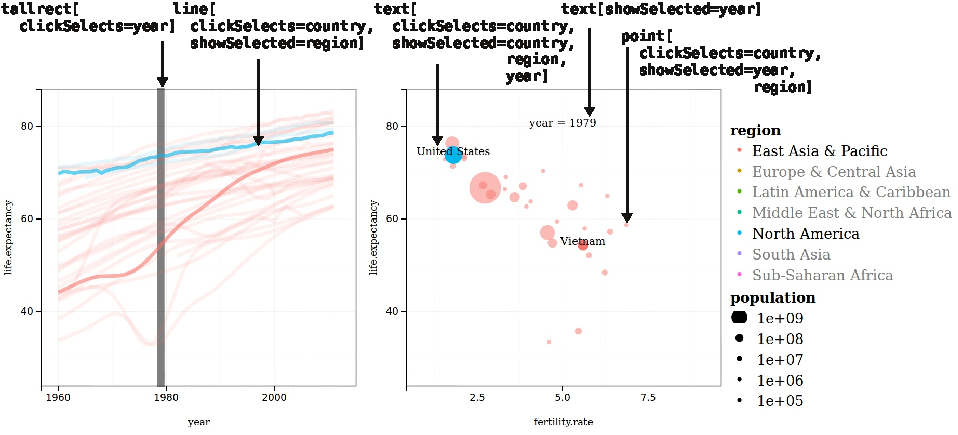
\includegraphics{images/figure-1}
\caption{\label{fig:worldbank}An interactive animation of World Bank
demographic data of several countries, designed using
\texttt{clickSelects} and \texttt{showSelected} aesthetics (top). Left:
a multiple time series from 1960 to 2010 of life expectancy, with bold
lines showing the selected countries and a vertical grey tallrect
showing the selected year. Right: a scatterplot of life expectancy
versus fertility rate of all countries. The legend and text elements
show the current selection: year=1979, country=\{United States,
Vietnam\}, and region=\{East Asia \& Pacific, North America\}}
\end{figure}

We anticipate that some \textbf{ggplot2} users will be able to reverse
engineer the code which creates Figure \ref{fig:worldbank}, simply by
looking at it. In fact, this is a big reason why \textbf{ggplot2} is so
widely used: it helps minimize the amount of time required to translate
an idea for a figure into computer code. Note that, in the left-hand
plot of Figure \ref{fig:worldbank}, we have a time series of the life
expectancy where each line is a country (i.e., we \texttt{group} by
country) and lines are colored by region. By clicking on a line, we also
want the country label to appear in the right-hand plot, so we also need
to set \texttt{clickSelects=country}. Lastly, by setting
\texttt{showSelected=region}, we can hide/show lines by clicking on the
color legend entries.

\begin{Shaded}
\begin{Highlighting}[]
\NormalTok{timeSeries <-}\StringTok{ }\KeywordTok{ggplot}\NormalTok{() }\OperatorTok{+}\StringTok{ }\KeywordTok{geom_line}\NormalTok{(}
  \DataTypeTok{data =}\NormalTok{ WorldBank,}
  \KeywordTok{aes}\NormalTok{(}\DataTypeTok{x =}\NormalTok{ year, }\DataTypeTok{y =}\NormalTok{ life.expectancy,}
      \DataTypeTok{group =}\NormalTok{ country, }\DataTypeTok{color =}\NormalTok{ region,}
      \DataTypeTok{clickSelects =}\NormalTok{ country, }
      \DataTypeTok{showSelected =}\NormalTok{ region)}
\NormalTok{)}
\end{Highlighting}
\end{Shaded}

We want to provide a visual cue for the selected year in the time
series, so in the code below we add some tall rectangles to the time
series plot. These tall rectangles will also serve as a way to directly
modify the selected year. The tallrect geometry is a special case of a
rectangle that automatically spans the entire vertical range, so we just
have to specify the horizontal range via \texttt{xmin} and \texttt{xmax}
aesthetics. Also, since the layered grammar of graphics allows for
different data in each layer, we supply a data frame with just the
unique years in the entire data for this layer.

\begin{Shaded}
\begin{Highlighting}[]
\NormalTok{years <-}\StringTok{ }\KeywordTok{data.frame}\NormalTok{(}\DataTypeTok{year =} \KeywordTok{unique}\NormalTok{(WorldBank}\OperatorTok{$}\NormalTok{year))}
\NormalTok{timeSeries <-}\StringTok{ }\NormalTok{timeSeries }\OperatorTok{+}\StringTok{ }\KeywordTok{geom_tallrect}\NormalTok{(}
  \DataTypeTok{data =}\NormalTok{ years,}
  \KeywordTok{aes}\NormalTok{(}\DataTypeTok{xmin =}\NormalTok{ year }\OperatorTok{-}\StringTok{ }\FloatTok{0.5}\NormalTok{, }\DataTypeTok{xmax =}\NormalTok{ year }\OperatorTok{+}\StringTok{ }\FloatTok{0.5}\NormalTok{,}
      \DataTypeTok{clickSelects =}\NormalTok{ year)}
\NormalTok{)}
\end{Highlighting}
\end{Shaded}

As for the right-hand plot in Figure \ref{fig:worldbank}, there are
three layers: a point layer for countries, a text layer for countries,
and a text layer to display the selected year. By clicking on a point,
we want to display the country text label and highlight the
corresponding time series on the left-hand plot, so we set
\texttt{clickSelects=country} in this layer. Furthermore, we only want
to show the points for the selected year and region, so we also need
\texttt{showSelected=year} and \texttt{showSelected2=region}.

\begin{Shaded}
\begin{Highlighting}[]
\NormalTok{scatterPlot <-}\StringTok{ }\KeywordTok{ggplot}\NormalTok{() }\OperatorTok{+}\StringTok{ }\KeywordTok{geom_point}\NormalTok{(}
  \DataTypeTok{data =}\NormalTok{ WorldBank,}
  \KeywordTok{aes}\NormalTok{(}\DataTypeTok{x =}\NormalTok{ fertility.rate, }\DataTypeTok{y =}\NormalTok{ life.expectancy,}
      \DataTypeTok{color =}\NormalTok{ region, }\DataTypeTok{size =}\NormalTok{ population,}
      \DataTypeTok{clickSelects =}\NormalTok{ country,}
      \DataTypeTok{showSelected =}\NormalTok{ year,}
      \DataTypeTok{showSelected2 =}\NormalTok{ region)}
\NormalTok{)}
\end{Highlighting}
\end{Shaded}

Note that any aesthetics containing the substring \texttt{showSelected}
(including \texttt{showSelected2}) are interpreted as
\texttt{showSelected} variables, and combined together using the
intersection operation. In the example above, that means that a point
will be drawn for the currently selected combination of year and region,
as in the following SQL query,

\begin{Shaded}
\begin{Highlighting}[]
\KeywordTok{SELECT}\NormalTok{ * }\KeywordTok{FROM}\NormalTok{ WorldBank}
  \KeywordTok{WHERE} \DataTypeTok{year}   \KeywordTok{IN}\NormalTok{ selected_year}
  \KeywordTok{AND}\NormalTok{   region }\KeywordTok{IN}\NormalTok{ selected_region}
\end{Highlighting}
\end{Shaded}

Below, the text layer for annotating selected countries is essentially
the same as the point layer, except we map the country name to the
\texttt{label} aesthetic.

\begin{Shaded}
\begin{Highlighting}[]
\NormalTok{scatterPlot <-}\StringTok{ }\NormalTok{scatterPlot }\OperatorTok{+}\StringTok{ }\KeywordTok{geom_text}\NormalTok{(}
  \DataTypeTok{data =}\NormalTok{ WorldBank,}
  \KeywordTok{aes}\NormalTok{(}\DataTypeTok{x =}\NormalTok{ fertility.rate, }\DataTypeTok{y =}\NormalTok{ life.expectancy,}
      \DataTypeTok{label =}\NormalTok{ country,}
      \DataTypeTok{showSelected =}\NormalTok{ country,}
      \DataTypeTok{showSelected2 =}\NormalTok{ year,}
      \DataTypeTok{showSelected3 =}\NormalTok{ region)}
\NormalTok{)}
\end{Highlighting}
\end{Shaded}

Lastly, to help identify the selected year when viewing the scatterplot,
we add another layer of text at a fixed location.

\begin{Shaded}
\begin{Highlighting}[]
\NormalTok{scatterPlot <-}\StringTok{ }\NormalTok{scatterPlot }\OperatorTok{+}\StringTok{ }\KeywordTok{geom_text}\NormalTok{(}
  \DataTypeTok{data =}\NormalTok{ years, }\DataTypeTok{x =} \DecValTok{5}\NormalTok{, }\DataTypeTok{y =} \DecValTok{80}\NormalTok{,}
  \KeywordTok{aes}\NormalTok{(}\DataTypeTok{label =} \KeywordTok{paste}\NormalTok{(}\StringTok{"year ="}\NormalTok{, year),}
      \DataTypeTok{showSelected =}\NormalTok{ year)}
\NormalTok{)}
\end{Highlighting}
\end{Shaded}

In summary, this section shows an example of how the proposed
\texttt{clickSelects} and \texttt{showSelected} aesthetics can be used
with several different geoms (line, point, text, tallrect), each of
which can potentially display a different data set. In each case we use
\texttt{clickSelects} to declare a geom for which clicking changes the
value of a selection variable, and we use \texttt{showSelected} to
declare a geom which responds to such changes by updating the set of
displayed data. In the next sections, we further explain how to link
ggplots and add animation.

\hypertarget{linking}{%
\subsection{Linking and multiple selection}\label{linking}}

Linking is declared in R code by putting ggplots with common
\texttt{clickSelects} and \texttt{showSelected} aesthetics together in a
list. For example, we can link the ggplots from the previous section by
including them together in the following list:

\begin{Shaded}
\begin{Highlighting}[]
\NormalTok{viz <-}\StringTok{ }\KeywordTok{list}\NormalTok{(}
  \DataTypeTok{timeSeries =}\NormalTok{ timeSeries,}
  \DataTypeTok{scatterPlot =}\NormalTok{ scatterPlot}
\NormalTok{)}
\end{Highlighting}
\end{Shaded}

Linking is accomplished because the two ggplots declared
\texttt{clickSelects} and \texttt{showSelected} aesthetics that refer to
common variable names (\texttt{region}, \texttt{year},
\texttt{country}). For each such selection variable, our interactive
renderer updates the set of selected values in response to mouse clicks
on \texttt{clickSelects} geoms, and then updates the corresponding data
which is displayed for \texttt{showSelected} geoms.

Note that the \texttt{viz} list above can also contain rendering
options, as we discuss below (see Table \ref{tab:overview} for a summary
of proposed interactive features). For example, the
\texttt{selector.types} option controls whether or not selections for a
given variable can accumulate (single or multiple selected values). This
difference is also sometimes referred to as transient versus persistent
selection (D. Cook and Swayne 2007).

\begin{Shaded}
\begin{Highlighting}[]
\NormalTok{viz}\OperatorTok{$}\NormalTok{selector.types <-}\StringTok{ }\KeywordTok{list}\NormalTok{(}
  \DataTypeTok{year =} \StringTok{"single"}\NormalTok{,}
  \DataTypeTok{country =} \StringTok{"multiple"}\NormalTok{,}
  \DataTypeTok{region =} \StringTok{"multiple"}
\NormalTok{)}
\end{Highlighting}
\end{Shaded}

The code above declares \texttt{year} as a single selection variable,
which means that only a single year may be selected at a time (clicking
a geom with \texttt{clickSelects=year} will change the selection to the
corresponding year). The \texttt{country} and \texttt{region} variables
are declared as multiple selection variables, which can have multiple
selected values at a time (clicking a geom with
\texttt{clickSelects=country} will add/remove that country to/from the
selection set).

\hypertarget{animation}{%
\subsection{Animation and smooth transitions}\label{animation}}

Animation is declared using the \texttt{time} option, which specifies a
selection variable that will be automatically updated over time, as well
as a time delay in milliseconds. The code below declares the
\texttt{year} variable to be animated every 3 seconds.

\begin{Shaded}
\begin{Highlighting}[]
\NormalTok{viz}\OperatorTok{$}\NormalTok{time <-}\StringTok{ }\KeywordTok{list}\NormalTok{(}\DataTypeTok{variable =} \StringTok{"year"}\NormalTok{, }\DataTypeTok{ms =} \DecValTok{3000}\NormalTok{)}
\end{Highlighting}
\end{Shaded}

Animation is useful in the World Bank data visualization because it
shows how the bi-variate relationship between fertility rate and life
expectancy changes over time. Animation clearly shows how many countries
progress from low life expectancy and high fertility rate in early
years, to high life expectancy and low fertility rate in later years.

Finally, the \texttt{duration} option specifies the amount of time used
to smoothly transition between selections (with linear easing). Smooth
transitions help the viewer track geoms before and after an update to
the selection set. For example in the code below we declare a 1 second
smooth transition on the \texttt{year} variable, in order to more easily
track the points on the scatterplot.

\begin{Shaded}
\begin{Highlighting}[]
\NormalTok{viz}\OperatorTok{$}\NormalTok{duration <-}\StringTok{ }\KeywordTok{list}\NormalTok{(}\DataTypeTok{year =} \DecValTok{1000}\NormalTok{)}
\end{Highlighting}
\end{Shaded}

Note that for accurate interpretation of smooth transitions, the new
\texttt{key} aesthetic must be specified. The \texttt{key} aesthetic is
used to match data elements before and after the smooth transition. In
the World Bank example, we would need to specify
\texttt{aes(key=country)} for the points and text in the scatterplot.

\hypertarget{compiling-and-rendering}{%
\subsection{Compiling and rendering}\label{compiling-and-rendering}}

We have implemented the \textbf{animint} R package which enables viewing
the linked interactive ggplots that we proposed in the previous
sections. Supplying the \texttt{viz} list of ggplots and rendering
options to the \texttt{animint2dir()} function will save all the files
necessary for rendering the visualization:

\begin{Shaded}
\begin{Highlighting}[]
\NormalTok{animint}\OperatorTok{::}\KeywordTok{animint2dir}\NormalTok{(viz)}
\end{Highlighting}
\end{Shaded}

As shown in supplementary Figure 1, the \textbf{animint} system is
implemented in 2 parts: the compiler and the renderer. The compiler is
implemented in R code that converts a list of ggplots and options to a
JSON plot meta-data file and a tab-separated values (TSV) file database.
The renderer consists of HTML and JavaScript files, which can be easily
hosted along with the TSV and JSON files on any web server. The
interactive plots can be viewed by opening the \texttt{index.html} page
in any modern web browser. Note that our current implementation of
\textbf{animint} depends on a fork of
\textbf{ggplot2}\footnote{\url{https://github.com/faizan-khan-iit/ggplot2/tree/validate-params}}
that contains some minor modifications which are needed to support
interactive rendering on web pages. Additional implementation details
are available in the supplementary materials.

\hypertarget{performance}{%
\section{Exploring scope with examples}\label{performance}}

This section attempts to demonstrate the range of visualizations that
are supported by the system we propose. In particular because of its
support for interaction and animation, it excels at display of
interactive maps with time-varying data. We give two such examples
below.

\hypertarget{tornadoes-in-the-united-states}{%
\subsection{Tornadoes in the United
States}\label{tornadoes-in-the-united-states}}

One of the strong points of the system we propose is display of
multi-layer plots such as maps with time-varying data. For example,
Figure \ref{fig:tornado} shows a visualization of US tornado data from
1950 to 2012. This data visualization consists of two multi-layer plots
with two interaction variables, \texttt{year} and \texttt{state}.

The left plot is a map which shows state borders using a polygon with
\texttt{clickSelects=state}. The currently selected state is shown using
semi-transparency, and other states can be selected by clicking them.
The state map plot uses geoms with \texttt{showSelected=year} to show
tornado paths (segment geom) and endpoints (point geom) for the
currently selected year (which is emphasized with a text geom above the
map).

The right plot uses several geoms to show details for the currently
selected state and year. A bar geom shows a time series of tornado
counts for the selected state (\texttt{showSelected=state}), which can
be clicked to change the currently selected year
(\texttt{clickSelects=year}). A text geom at the top of the plot shows
the currently selected state (\texttt{showSelected=state}), and a text
geom at the bottom emphasizes the tornado count for the selected year
(using \texttt{showSelected} variables for both \texttt{state} and
\texttt{year}).

These interactions can be useful for discovering patterns in the data,
and for suggesting models that can describe or predict tornado paths.

\begin{figure}
\centering
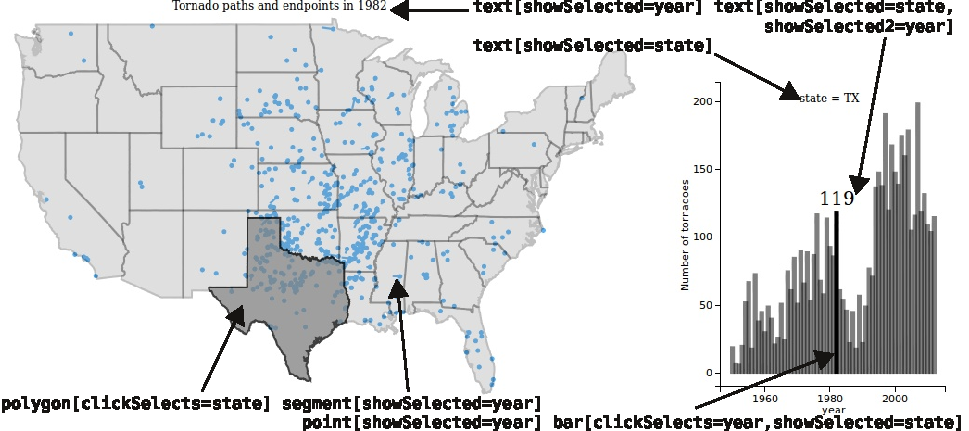
\includegraphics{images/figure-tornado}
\caption{\label{fig:tornado}Interactive animation of US tornadoes from 1950
to 2012. This figure depicts a scenario where the user queried Texas (by
clicking the map), and the year 1982 (by clicking the bar chart). In
addition to the graphical elements being highlighted as a visual clue of
what query is being made, this visualization includes dynamic text
labels reflecting the query.}
\end{figure}

\hypertarget{central-american-climate-data}{%
\subsection{Central American climate
data}\label{central-american-climate-data}}

\begin{figure}
\centering
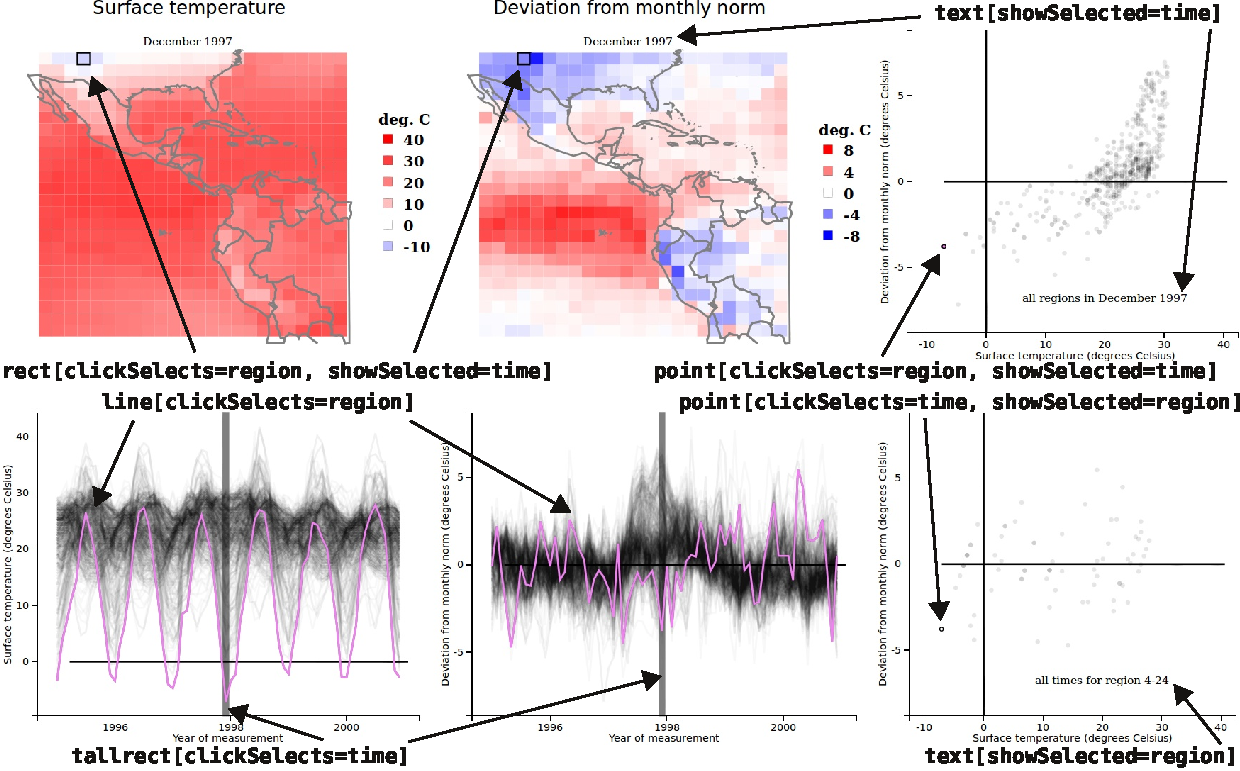
\includegraphics{images/figure-climate}
\caption{\label{fig:climate}Visualization containing 6 linked, interactive,
animated plots of Central American climate data. Top: for the selected
time (December 1997), maps displaying the spatial distribution of two
temperature variables, and a scatterplot of these two variables. The
selected region is displayed with a black outline, and can be changed by
clicking a rect on the map or a point on the scatterplot. Bottom: time
series of the two temperature variables with the selected region shown
in violet, and a scatterplot of all times for that region. The selected
time can be changed by clicking a background tallrect on a time series
or a point on the scatterplot. The selected region can be changed by
clicking a line on a time series.}
\end{figure}

A more complex map data visualization example is shown in Figure
\ref{fig:climate}, which depicts climate time series data observed in
Central America. There are two interaction variables, \texttt{time} and
\texttt{region}.

Two maps in the upper left display borders of the countries in and near
Central America. Unlike the previous example with US states, the country
borders are static (clicking has no effect). For the currently selected
time, rect geoms with \texttt{showSelected=time} show the spatial
distribution of sea surface temperature as well as its deviation from
the monthly norm. Since \texttt{clickSelects=region} is specified,
clicking a rect changes the currently selected region, which is
emphasized with a black border. These plots facilitate visualization of
the spatial distribution of the climate variables, and how they change
over time.

The plots below the maps use lines to show time series of the climate
variables. Since \texttt{clickSelects=region} is specified, clicking a
line changes the currently selected region, which is emphasized with a
purple color. A semi-transparent tallrect shows the currently selected
time; other tallrects can be clicked to update the time
(\texttt{clickSelects=time}). These plots make it easy to select
different times and regions, and to make comparisons between times and
regions.

Scatterplots on the right use \texttt{showSelected} variables with point
and text geoms, to show the joint distribution of the two temperature
variables for the selected time (top) and region (bottom). The plots use
\texttt{clickSelects} to emphasize the currently selected region (top)
and time (bottom), and are useful for visualizing normality and outliers
in the joint distribution.

\hypertarget{compare}{%
\section{Comparison study}\label{compare}}

In this section we compare our \textbf{animint} implementation with
other similar leading systems by creating a given visualization in each
system and discussing the pros and cons of the different approaches.

\hypertarget{tour}{%
\subsection{The Grand Tour}\label{tour}}

The Grand Tour is a well-known method for viewing high dimensional data
which requires interactive and dynamic graphics (Asimov 1985). Figure
\ref{fig:tour} shows a grand tour of 300 observations sampled from a
correlated tri-variate normal distribution. The left-hand view shows the
marginal density of each point while the right-hand view ``tours''
through 2D projections of the 3D data. There are many ways to choose
projections in a tour, and many ways to interpolate between projections,
most of which can be programmed fairly easily using R and relevant
add-on packages. In this case, we used the R package \textbf{tourr},
which uses the geodesic random walk (i.e., random 2D projection with
geodesic interpolation) in its grand tour algorithm (Wickham et al.
2011).

\begin{figure}
\centering
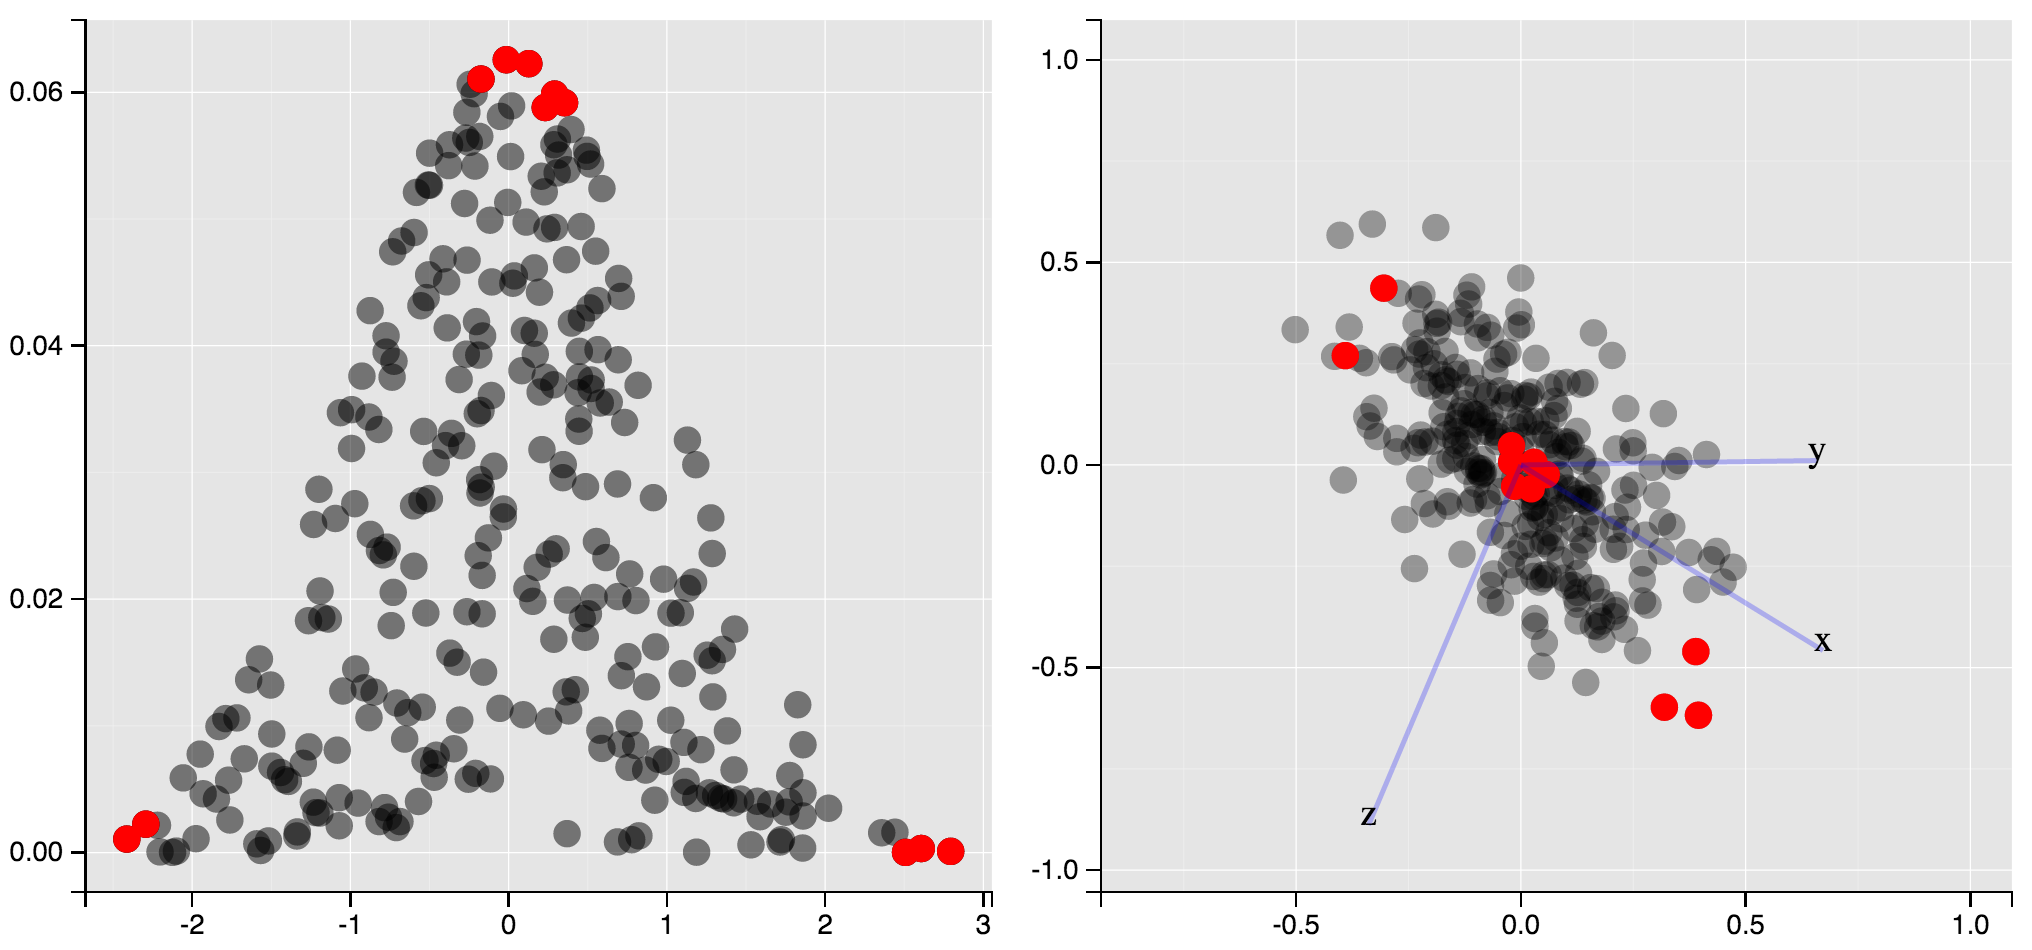
\includegraphics{images/tour}
\caption{\label{fig:tour}Linked selection in a grand tour with
\textbf{animint}. A video demonstration can be viewed online at
\url{https://vimeo.com/160720834}}
\end{figure}

When touring data, it is generally useful to link low-dimensional
displays with the tour itself. The video in Figure \ref{fig:tour} was
generated with our current \textbf{animint} implementation, and points
are selected via mouse click which reveals that points with high
marginal density are located in the ellipsoid center while points with a
low marginal density appear near the ellipsoid border. In this case, it
would be convenient to also have brush selection, as we demonstrate in
Figure \ref{fig:tourbrush} which implements the same touring example
using the R packages \textbf{ggvis} and \textbf{shiny}. The brush in
Figure \ref{fig:tourbrush} is implemented with \textbf{shiny}'s support
for brushing static images, which currently does not support multiple
brushes, making it difficult to select non-contiguous regions.

\begin{figure}
\centering
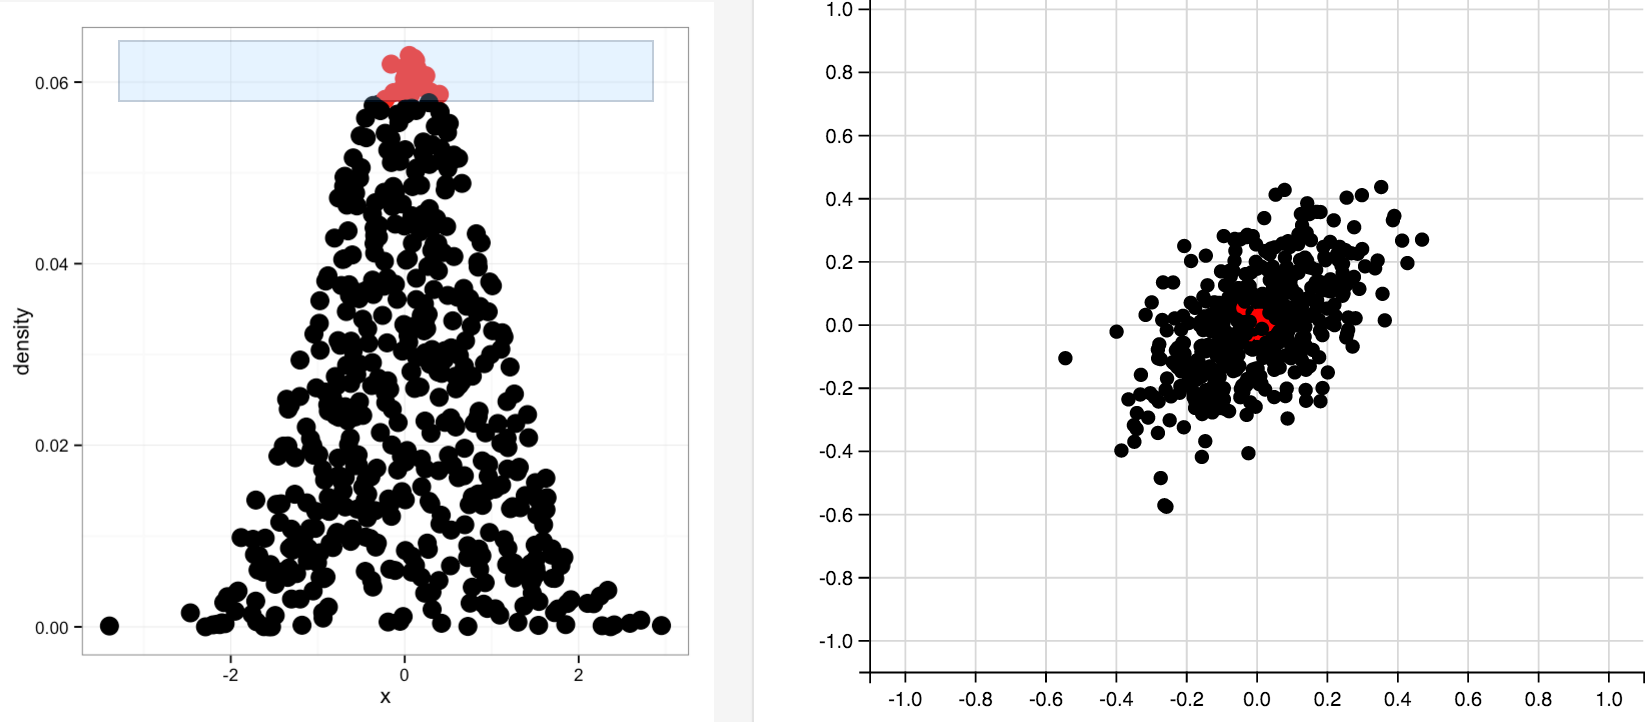
\includegraphics{images/tourbrush}
\caption{\label{fig:tourbrush}Linked selection in a grand tour with
\textbf{ggvis} and \textbf{shiny}. A video demonstration can be viewed
online at \url{https://vimeo.com/160825528}}
\end{figure}

This example helps point out a few other important differences in using
\textbf{animint} versus \textbf{ggvis}+\textbf{shiny} to implement
``multiple linked and dynamic views'' as described in Ahlberg,
Williamson, and Shneiderman (1991) and Buja et al. (1991). Maintaining
state of the linked brush in Figure \ref{fig:tourbrush} requires both
knowledge and clever use of some sophicated programming techniques such
as closures and reactivity. It also requires knowledge of the
\textbf{shiny} web application framework and a new approach to the
Grammar of Graphics. On the other hand, maintaining state in Figure
\ref{fig:tour} requires a few different
\texttt{clickSelects}/\texttt{showSelected} mappings. As a result, we
believe \textbf{animint} provides a more elegant user interface for this
application.

The touring example also helps point out important consequences of the
design and implementation of these two different systems. As mentioned
in Section \ref{implementation}, our current \textbf{animint}
implementation requires every subset of data to be precomputed before
render time. For visualizations such as tours, where it is more
efficient to perform statistical computations on-the-fly, this can be a
harsh restriction, but this is a restriction of our current
implementation (not a restriction of the framework itself). As a result,
when touring a large high-dimensional space, where many projections are
needed, \textbf{ggvis}+\textbf{shiny} may be desirable since the
projections are computed on the server and sent to the browser in
real-time. This works fine when the application is running and viewed on
the same host machine, but viewing such an application hosted on a
remote machine can produce staggered animations since client-server
requests must be performed, processed, and rendered roughly 30 times a
second. Also, generally speaking, the \textbf{animint} system results a
more pleasant experience when it comes to hosting and sharing
applications since it doesn't require a Web Server with R and special
software already installed.

\hypertarget{world-bank-example}{%
\subsection{World Bank example}\label{world-bank-example}}

We also recreated Figure \ref{fig:worldbank} using
\textbf{ggvis}+\textbf{shiny} and Tableau. Even as experienced
\textbf{ggvis}+\textbf{shiny} users, we found it quite difficult to
replicate this example, and were not able to completely replicate it due
to a lack of a mechanism for coordinating indirect and direct
manipulations. Overall the visualization is pretty similar, but lacks a
few important features. In particular, there is no way to control the
selected year using both the slider (indirect) and clicking on the
\textbf{ggvis} plot (direct). It also lacks the ability to click on a
country time series and label the corresponding point on the
scatterplot. This might be possible, but we could not find a way to
update a plot based on a click event on a different plot. Even with this
lack of functionality, the \textbf{ggvis}+\textbf{shiny} is
significantly more complicated and requires more code (about 100 lines
of code compared to 30).

It was also impossible to completely replicate Figure
\ref{fig:worldbank} using Tableau essentially because the example
requires a \emph{layered} approach to the Grammar of Graphics. In
particular, since graphical marks and interaction source/target(s) must
derive from the same table in Tableau, it was impossible to control the
clickable multiple time series and the clickable tallrects in different
ways based on the two different selection variables. In other words, in
Tableau, selections are managed on the plot level, but in
\textbf{animint}, selections are specific to each graphical layer.

\hypertarget{limitations}{%
\section{Limitations and future work}\label{limitations}}

The system we have proposed provides linked interactive plots via the
new \texttt{showSelected} and \texttt{clickSelects} aesthetics. The
linking between plots is rather flexible, but is limited to interactions
which are specified by the plot designer at compile-time. Our current
implementation provides a visual indication of the current selection via
semi-transparency of \texttt{clickSelects} geoms. In future work we
would like to explore more obvious visual cues that can be used to
quickly show the user the links between plots and possible interactions.

A number of limitations in our current implementation derive from the
fact that some plot features are computed once during the compilation
step, and remain static on a rendered plot. For example, users are
unable to change variable mappings after compilation. Also, when
different data subsets have very different ranges of values, it may be
preferable to recompute scales when \texttt{clickSelects} selection(s)
change. Some of these limitations can be resolved by adding interactive
widgets to ``recompile'' components hard-coded in the plot meta
information. In fact, \textbf{animint} makes it easy to embed
visualizations inside of \textbf{shiny} web applications, and we have an
example of interactively redefining variable mappings.

Our compiler also currently takes advantage of \textbf{ggplot2}
internals to compute statistics and positional adjustments before
rendering. As a result, statistics/positions will not dynamically
recompute based on selections. In other words, using
\texttt{clickSelects}/\texttt{showSelected} with non-identity
statistic(s)/position(s) may not generate a sensible result. It would be
possible, but a significant amount of work, to transfer these
computations from the compiler to the renderer.

Another set of limitations derive from our current restriction that all
subsets (corresponding to each possible selection) must be precomputed
before render time. As elucidated in Section \ref{tour}, if there is a
large space of possible selections, it is impractical to precompute
every subset before viewing. Therefore, for future work it would be
useful if the renderer could dynamically compute subsets when new
selections are made.

Our implementation is also limited to two specific types of direct
manipulation: selecting graphical elements via mouse click
(\texttt{clickSelects}), and showing/hiding related elements
(\texttt{showSelected}). However, the framework described in Section
\ref{extension} is not restricted to a particular event type, so
\texttt{hoverSelects} and \texttt{brushSelects} aesthetics could be
added, for instance. There are other types of interaction that could be
added, that wouldn't require additional extensions to the Grammar of
Graphics, such as: zooming, panning, and plot resizing.

\hypertarget{conclusion}{%
\section{Conclusion}\label{conclusion}}

We have proposed several extensions to \textbf{ggplot2}'s layered
grammar of graphics in order to support a declarative approach to
producing interactive and dynamic web graphics. By adding
\texttt{clickSelects} and \texttt{showSelected} aesthetics to specify
selection source(s) and target(s), \textbf{ggplot2} users can quickly
and easily create animations with smooth transitions and perform dynamic
queries via direct manipulation of linked views. As a result,
\textbf{animint} is a useful tool not only for EDA, but also for the
presentation and distribution of interactive statistical graphics.

\section*{Interactive figures and reproducible research statement}

The source code to create this paper and its figures is online at
\url{https://github.com/tdhock/animint-paper/} and the interactive
figures can be viewed at
\url{http://members.cbio.mines-paristech.fr/~thocking/animint-paper-figures/}

\section*{Acknowledgements}

The authors wish to thank \textbf{animint} users MC Du Plessis, Song
Liu, Nikoleta Juretic, and Eric Audemard who have contributed
constructive criticism and helped its development.

\section*{References}

\hypertarget{refs}{}
\leavevmode\hypertarget{ref-Ahlberg:1991}{}%
Ahlberg, Christopher, Christopher Williamson, and Ben Shneiderman. 1991.
``Dynamic Queries for Information Exploration: An Implementation and
Evaluation.'' In \emph{ACM Chi '92 Conference Proceedings}, 21:619--26.

\leavevmode\hypertarget{ref-viewing-pipeline}{}%
Andreas Buja, Catherine Hurley, Daniel Asimov, and John A. McDonald.
1988. ``Elements of a Viewing Pipeline for Data Analysis.'' In
\emph{Dynamic Graphics for Statistics}, edited by William S. Cleveland
and Marylyn E. McGill. Belmont, California: Wadsworth, Inc.

\leavevmode\hypertarget{ref-grand-tour}{}%
Asimov, Daniel. 1985. ``The Grand Tour: A Tool for Viewing
Multidimensional Data.'' \emph{SIAM J. Sci. Stat. Comput.} 6 (1).
Philadelphia, PA, USA: Society for Industrial; Applied
Mathematics:128--43. \url{https://doi.org/10.1137/0906011}.

\leavevmode\hypertarget{ref-brushing-scatterplots}{}%
Becker, RA, and WS Cleveland. 1987. ``Brushing Scatterplots.''
\emph{Technometrics} 29 (2):127--42.

\leavevmode\hypertarget{ref-trellis}{}%
Becker, Richard A., William S. Cleveland, and Ming-Jen Shyu. 2010. ``The
Visual Design and Control of Trellis Displays.'' \emph{Journal of
Computational and Graphical Statistics} 19 (1). Taylor \& Francis:3--28.

\leavevmode\hypertarget{ref-d3}{}%
Bostock, Michael, Vadim Oglevetsky, and Jeffrey Heer. 2011. ``D3
Data-Driven Documents.'' \emph{IEEE Transactions on Visualization and
Computer Graphics} 17 (12):2301--9.

\leavevmode\hypertarget{ref-Buja:1991vh}{}%
Buja, Andreas, John Alan McDonald, John Michalak, and Werner Stuetzle.
1991. ``Interactive data visualization using focusing and linking.''
\emph{IEEE Proceedings of Visualization}, February, 1--8.

\leavevmode\hypertarget{ref-cairo}{}%
Cairo. 2016. ``Cairo: A Vector Graphics Library.''
\url{http://cairographics.org/}.

\leavevmode\hypertarget{ref-ggvis}{}%
Chang, Winston, and Hadley Wickham. 2015. \emph{ggvis: Interactive
Grammar of Graphics}. \url{https://CRAN.R-project.org/package=ggvis}.

\leavevmode\hypertarget{ref-Cook:2007uk}{}%
Cook, Dianne, Andreas Buja, and Deborah F Swayne. 2007. ``Interactive
High-Dimensional Data Visualization.'' \emph{Journal of Computational
and Graphical Statistics}, December, 1--23.

\leavevmode\hypertarget{ref-ggobi:2007}{}%
Cook, Dianne, and Deborah F. Swayne. 2007. \emph{Interactive and Dynamic
Graphics for Data Analysis : With R and GGobi}. Use R ! New York:
Springer. \url{http://www.ggobi.org/book/}.

\leavevmode\hypertarget{ref-rggobi}{}%
Duncan Temple Lang, Hadley Wickham, Debby Swayne. 2016. \emph{Interface
Between R and GGobi}.

\leavevmode\hypertarget{ref-PRIM9}{}%
Fisherkeller, Friedman, M. A., and J. W. Tukey. 1988. ``PRIM-9, an
Interactive Multidimensional Data Display and Analysis System.'' In
\emph{Dynamic Graphics for Statistics}, 91--109.

\leavevmode\hypertarget{ref-qtbase}{}%
Lawrence, Michael, and Deepayan Sarkar. 2016. \emph{Interface Between R
and Qt}. \url{https://github.com/ggobi/qtbase}.

\leavevmode\hypertarget{ref-RGtk2}{}%
Lawrence, Michael, and Duncan Temple Lang. 2010. ``RGtk2: A Graphical
User Interface Toolkit for R.'' \emph{Journal of Statistical Software}
37 (8):1--52. \url{http://www.jstatsoft.org/v37/i08/}.

\leavevmode\hypertarget{ref-gridSVG}{}%
Murrell, Paul, and Simon Potter. 2015. \emph{gridSVG: Export 'grid'
Graphics as SVG}. \url{https://CRAN.R-project.org/package=gridSVG}.

\leavevmode\hypertarget{ref-SVGAnnotation}{}%
Nolan, Deborah, and Duncan Temple Lang. 2012. ``Interactive and Animated
Scalable Vector Graphics and R Data Displays.'' \emph{Journal of
Statistical Software} 46 (1):1--88.
\url{http://www.jstatsoft.org/v46/i01/}.

\leavevmode\hypertarget{ref-plotly}{}%
Plotly. 2015. ``Collaborative Data Science.'' Montreal, QC: Plotly
Technologies Inc. 2015. \url{https://plot.ly}.

\leavevmode\hypertarget{ref-RCore}{}%
R Core Team. 2017. \emph{R: A Language and Environment for Statistical
Computing}. Vienna, Austria: R Foundation for Statistical Computing.
\url{http://www.R-project.org/}.

\leavevmode\hypertarget{ref-gganimate}{}%
Robinson, David. 2016. \emph{gganimate: Create easy animations with
ggplot2}. \url{http://github.com/dgrtwo/gganimate}.

\leavevmode\hypertarget{ref-shiny}{}%
RStudio. 2013. ``Shiny: Easy Web Applications in R.''
\url{http://www.rstudio.com/shiny/}.

\leavevmode\hypertarget{ref-xgobi}{}%
Swayne, DF, D Cook, and A Buja. 1998. ``XGobi: Interactive Dynamic Data
Visualization in the X Window System.'' \emph{Journal of Computational
and Graphical Statistics} 7 (1):113--30.

\leavevmode\hypertarget{ref-mondrian}{}%
Theus, M. 2002. ``Interactive Data Visualization Using Mondrian.''
\emph{Journal of Statistical Software} 7 (11):1--9.
\url{http://www.jstatsoft.org/v07/i11}.

\leavevmode\hypertarget{ref-LISP-STAT}{}%
Tierney, Luke. 1990. \emph{LISP-Stat: An Object Oriented Environment for
Statistical Computing and Dynamic Graphics.} Wiley-Interscience, New
York.

\leavevmode\hypertarget{ref-vega}{}%
Trifacta. 2014. ``Vega: A Declarative Visualization Grammar.''
\url{http://trifacta.github.io/vega/}.

\leavevmode\hypertarget{ref-Unwin:1999vp}{}%
Unwin, Antony, and Heike Hofmann. 2009. ``GUI and Command-line -
Conflict or Synergy?'' \emph{Proceedings of the St Symposium on the
Interface}, September, 1--11.

\leavevmode\hypertarget{ref-MANET}{}%
Unwin A., Hofmann H., Hawkins G. 1996. ``Interactive Graphics for Data
Sets with Missing Values - Manet.'' \emph{Journal of Computational and
Graphical Statistics} 4 (6).

\leavevmode\hypertarget{ref-Urbanek2011}{}%
Urbanek, Simon. 2011. ``IPlots eXtreme: Next-Generation Interactive
Graphics Design and Implementation of Modern Interactive Graphics.''
\emph{Computational Statistics} 26 (3):381--93.
\url{https://doi.org/10.1007/s00180-011-0240-x}.

\leavevmode\hypertarget{ref-rJava}{}%
---------. 2016. \emph{rJava: Low-level R to Java Interface}.
\url{https://CRAN.R-project.org/package=rJava}.

\leavevmode\hypertarget{ref-htmlwidgets}{}%
Vaidyanathan, Ramnath, Yihui Xie, JJ Allaire, Joe Cheng, and Kenton
Russell. 2018. \emph{htmlwidgets: HTML Widgets for R}.
\url{https://github.com/ramnathv/htmlwidgets}.

\leavevmode\hypertarget{ref-loon}{}%
Waddell, Adrian, and R. Wayne Oldford. 2018. \emph{loon: Interactive
Statistical Data Visualization}.
\url{https://CRAN.R-project.org/package=loon}.

\leavevmode\hypertarget{ref-ggplot2-paper}{}%
Wickham, Hadley. 2010. ``A Layered Grammar of Graphics.'' \emph{Journal
of Computational and Graphical Statistics} 19 (1). Taylor \&
Francis:3--28.

\leavevmode\hypertarget{ref-tourr}{}%
Wickham, Hadley, Dianne Cook, Heike Hofmann, and Andreas Buja. 2011.
``tourr: An R Package for Exploring Multivariate Data with
Projections,'' April, 1--18.

\leavevmode\hypertarget{ref-plumbing}{}%
Wickham, Hadley, Michael Lawrence, Dianne Cook, Andreas Buja, Heike
Hofmann, and Deborah F Swayne. 2010. ``The Plumbing of Interactive
Graphics.'' \emph{Computational Statistics}, April, 1--7.

\leavevmode\hypertarget{ref-animation}{}%
Xie, Yihui. 2013. ``animation: An R Package for Creating Animations and
Demonstrating Statistical Methods.'' \emph{Journal of Statistical
Software} 53 (1):1--27. \url{http://www.jstatsoft.org/v53/i01/}.

\leavevmode\hypertarget{ref-cranvas}{}%
Xie, Yihui, Heike Hofmann, Di Cook, Xiaoyue Cheng, Barret Schloerke,
Marie Vendettuoli, Tengfei Yin, Hadley Wickham, and Michael Lawrence.
2013. \emph{Interactive Statistical Graphics Based on Qt}.



\end{document}
